\subsection{Rangefinder Implementation}
With the data acquisition command tested and functioning properly, the rangefinder needs to be connected to the ZedBoard. Since the URG-04LX uses UART communication, there are a few reasonable options to create a UART controller on the ZedBoard.

\subsubsection{UART Options}
As the ZedBoard is such a powerful device, it has a few different options for controlling UART. A few of them are by controlling UART through linux, through a MicroBlaze soft-core processor, or through the Zynq-7000 Processing System. Running linux on the ZedBoard would use much of the board's valuable resources, and we would only be using a fraction of the capability provided by linux. The MicroBlaze soft-core processor would be a better alternative, but it runs in the programmable logic in the FPGA and is unnecessary when the ARM processor on the ZedBoard is unused \cite{microblaze}. Because of this, we decided to utilize the ARM processor on the ZedBoard by using the Zynq7 Processing System via Xilinx's Zynq-7000 Processing System Intellectual Property (IP) core.

\subsubsection{Zynq7 Processing System}
The ZedBoard SoC features a dual-core ARM Cortex-A9 MPCore processing system and Xilinx Programmable Logic. The Zynq7 Processing System IP core acts as a logic interface that integrates the Programmable Software (PS) with the Programmable Logic (PL), which allows access to both on-chip and external memory interfaces, to PL clocks, to many I/O peripherals, and even to extended I/O peripherals \cite{zynq7ps}. With all of this overwhelming functionality, the processing system is easy to customize, featuring a simple user interface, once it is added into a project's block design. The user interface can be used to change the processing system's activated features. Figure \ref{zynq7ps_pic} below shows the processing system customization window.

\begin{figure}[H]
	\centerline{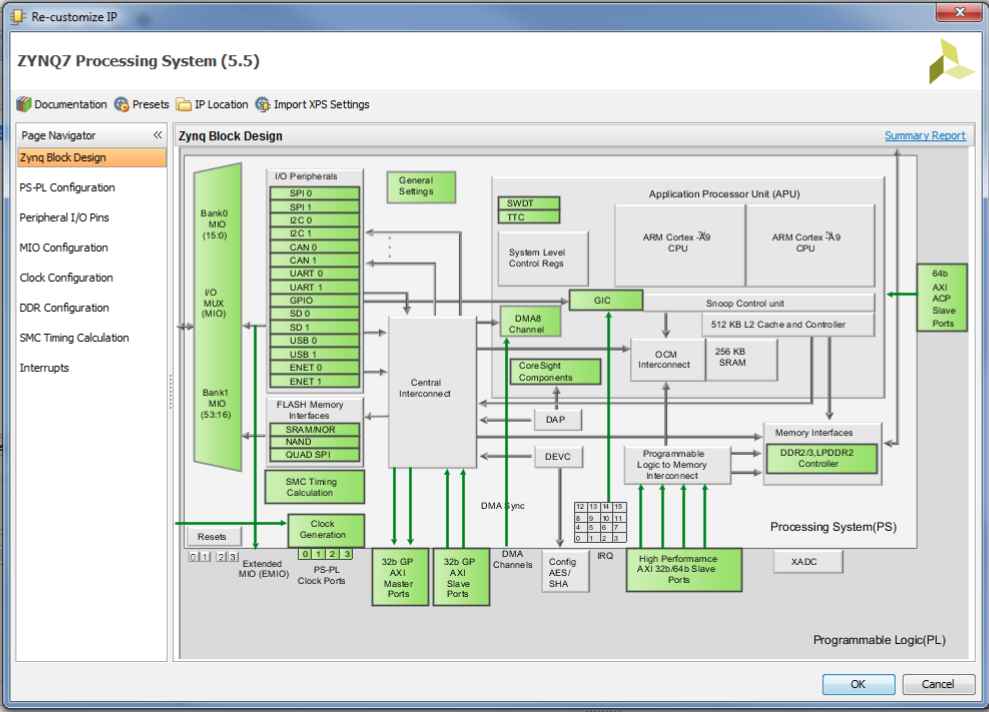
\includegraphics[width=1\textwidth]{zynq7ps.png}}
	\caption{Zynq7 Processing System Customization Window \cite{zynq7ps}}
	\label{zynq7ps_pic}
\end{figure}

In the figure above there are two options for UART shown: UART0 and UART1. The functionality of UART0 and UART1 are nearly identical, except that UART1 has the capability of being routed to the ZedBoard's USB UART port, which is not compatible with the rangefinder \cite{zedboard_datasheet}. So, we arbitrarily chose UART0 and routed the signals to MIO10 and MIO11, which correspond to the ZedBoard's PS Pmod, JE.
\par
After choosing UART0 and configuring the MIO pins, the Baud Rate needs to be configured such that it corresponds with the rangefinder's default communication speed, 19200 Baud \cite{urg04lx_datasheet}. This can be done in the processing system's customization window under PS-PL Configuration on the sidebar in Figure \ref{zynq7ps_pic}. Figure \ref{zynq7ps_baud_pic} below shows the PS-PL Configuration window.

\begin{figure}[H]
	\centerline{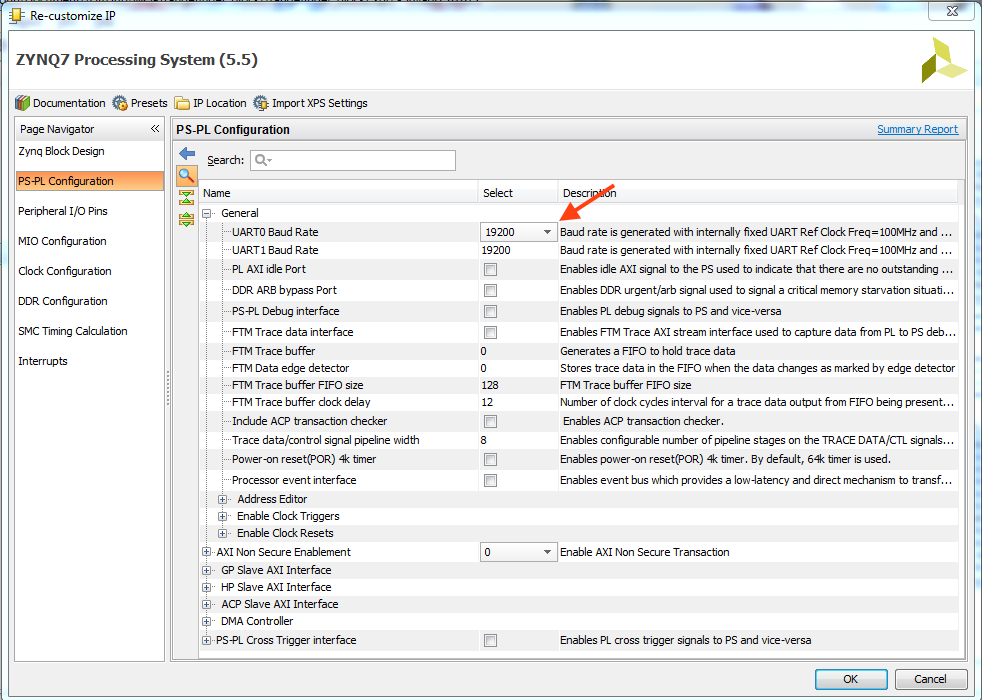
\includegraphics[width=1\textwidth]{zynq7ps_baud.png}}
	\caption{Zynq7 Processing System PS-PL Configuration Window}
	\label{zynq7ps_baud_pic}
\end{figure}

With the processing system customized in this fashion, the programmable logic's configuration is complete.

\subsubsection{PS-PL Communication / Creating Custom IP}
\label{sssec:ps_pl}
I HAVE NO IDEA WHAT TO WRITE FOR THIS